\documentclass{../source/Experiment}

\major{信息工程}
\name{}
\title{戴维南定理的实验研究}
\stuid{}
\college{信息与电子工程学院}
\date{\today}
\lab{东4-216}
\course{电子电路设计实验}
\instructor{李锡华、施红军、叶险峰}
\grades{}
\expname{戴维南定理的实验研究}
\exptype{研究实验}
\partner{}

\begin{document}
    \makecover
    \makeheader

    \section{实验目的}
        \begin{enumerate}
            \item 实验研究戴维南定理;
            \item 掌握有源二端口网络等效电路参数的测量方法。
        \end{enumerate}
    \section{实验任务和要求}
        \begin{enumerate}
            \item 按电路图连接好待测电路。
            \item 测量戴维南等效电压和等效电阻。
            \item 用等效电路进行戴维南定理的验证。
        \end{enumerate}
    \section{实验方案设计与实验参数计算}
        \subsection{完整的实验电路}
            \begin{figure}[htbp]
                \begin{center}
                    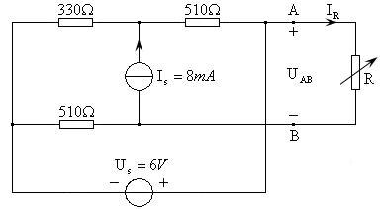
\includegraphics[scale=0.8]{pic/pic3.png}
                    \caption{戴维南定理实验电路}
                \end{center}
            \end{figure}
                \newpage
            \begin{figure}[htbp]
                \begin{center}
                    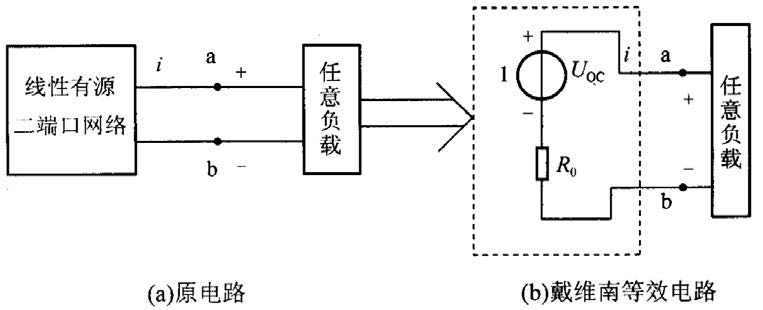
\includegraphics[scale=0.8]{pic/pic4.jpg}
                    \caption{戴维南定理等效电路}
                \end{center}
            \end{figure}
        \subsection{实验方案总体设计}
            \begin{enumerate}
                \item 接入稳压电源$U_S = 6V$和恒流源$I_s = 8mA$,接入负载$R_L$。测出$U_{OC}$和$I_{SC}$,并计算出$R_O$,填表。
                \item 负载实验:接入负载$R_L$,改变$R_L$阻值,测量有源二端口网络的外特性,将实验数据填入表中。对$U-I$进行作图。
                \item 验证戴维南定理:用一只1k$\Omega$的电位器作为$R_O$,将其阻值调整到等于步骤(1)所得的等效电阻$R_O$的值,然后令其与直流稳压电源$U_{OC}$(即步骤(1)所测得的开路电压值)相串联,按图2进行实验,将实验数据填入表中,作图对戴维南定理进行验证。
            \end{enumerate}
    \section{主要仪器设备}
            万用表,电压源,恒定电流源,电阻若干,电位器,电流表。
    \section{实验步骤、实验调试过程、实验数据记录}
        \subsection{实验步骤以及实验调试过程}
            \begin{enumerate}
                \item 按电路图1连接好电路。接入稳压电源$U_S = 6V$和恒流源$I_s = 8mA$,接入负载$R_L$。测出$U_{OC}$和$I_{SC}$,并计算出$R_O$,填表1。
                \item 负载实验:接入负载$R_L$,改变$R_L$阻值,测量有源二端口网络的外特性,将实验数据填入表中。对$U-I$进行作图。
                \item $U_1$处不接电源,将节点 F,E 之间短路,在节点 B,C 之间接入电压源 $U_2$,再次测量各点电压与各支路电流,记入表2中。
                \item 验证戴维南定理:用一只1k$\Omega$的电位器作为$R_O$,将其阻值调整到等于步骤(1)所得的等效电阻$R_O$的值,然后令其与直流稳压电源$U_{OC}$(即步骤(1)所测得的开路电压值)相串联,按图2进行实验,将实验数据填入表中,作图对戴维南定理进行验证。
            \end{enumerate}
        \subsection{实验数据记录}
            \newpage
            \begin{table}[htbp]
                \begin{center}
                    \caption{实验数据}
                    \begin{tabular}{|c|c|c|}
                        \hline
                        $U_{OC}(V)$ & $I_{SC}(mA)$ & $R_O = U_{OC}/I_{SC}(\Omega)$ \\           
                        \hline
                        10.02 & 19.71 & 508.37 \\
                        \hline
                    \end{tabular}
                    \caption{实验数据记录}
                    \begin{tabular}{|c|c|c|c|c|c|c|c|c|c|}
                        \hline
                        $R_L(\Omega)$ & 16.8 & 86.7 & 205 & 284 & 480 & 662 & 1127 & 1771 & 3470 \\
                        \hline
                        $U_{AB}(V)$ & 0.285 & 1.418 & 2.84 & 3.55 & 4.81 & 5.64 & 6.88 & 7.78 & 8.76 \\
                        \hline
                        $I(mA)$ & 18.89 & 16.86 & 14.14 & 12.76 & 10.24 & 8.70 & 6.24 & 4.49 & 2.56 \\
                        \hline
                    \end{tabular}
                    \caption{实验数据记录}
                    \begin{tabular}{|c|c|c|c|c|c|c|c|c|c|}
                        \hline
                        $R_L(\Omega)$ & 17.3 & 95.1 & 196 & 310 & 449 & 635 & 1059 & 1763 & 3060 \\
                        \hline
                        $U_{AB}(V)$ & 0.313 & 1.552 & 2.76 & 3.69 & 4.58 & 5.46 & 6.70 & 7.78 & 8.61 \\
                        \hline
                        $I(mA)$ & 19.10 & 16.70 & 14.30 & 12.09 & 10.47 & 8.78 & 6.45 & 4.48 & 2.86 \\
                        \hline
                    \end{tabular}
                \end{center}
            \end{table}
    \section{实验结果和分析处理}
        \subsection{数据分析}
        将表2和表3的数据进行线性拟合后,对比两图像可知,再误差允许范围内,原电路可以等效为戴维南等效电路。
        \begin{figure}[htbp]          
            \begin{minipage}[t]{0.5\textwidth}
                \centering
                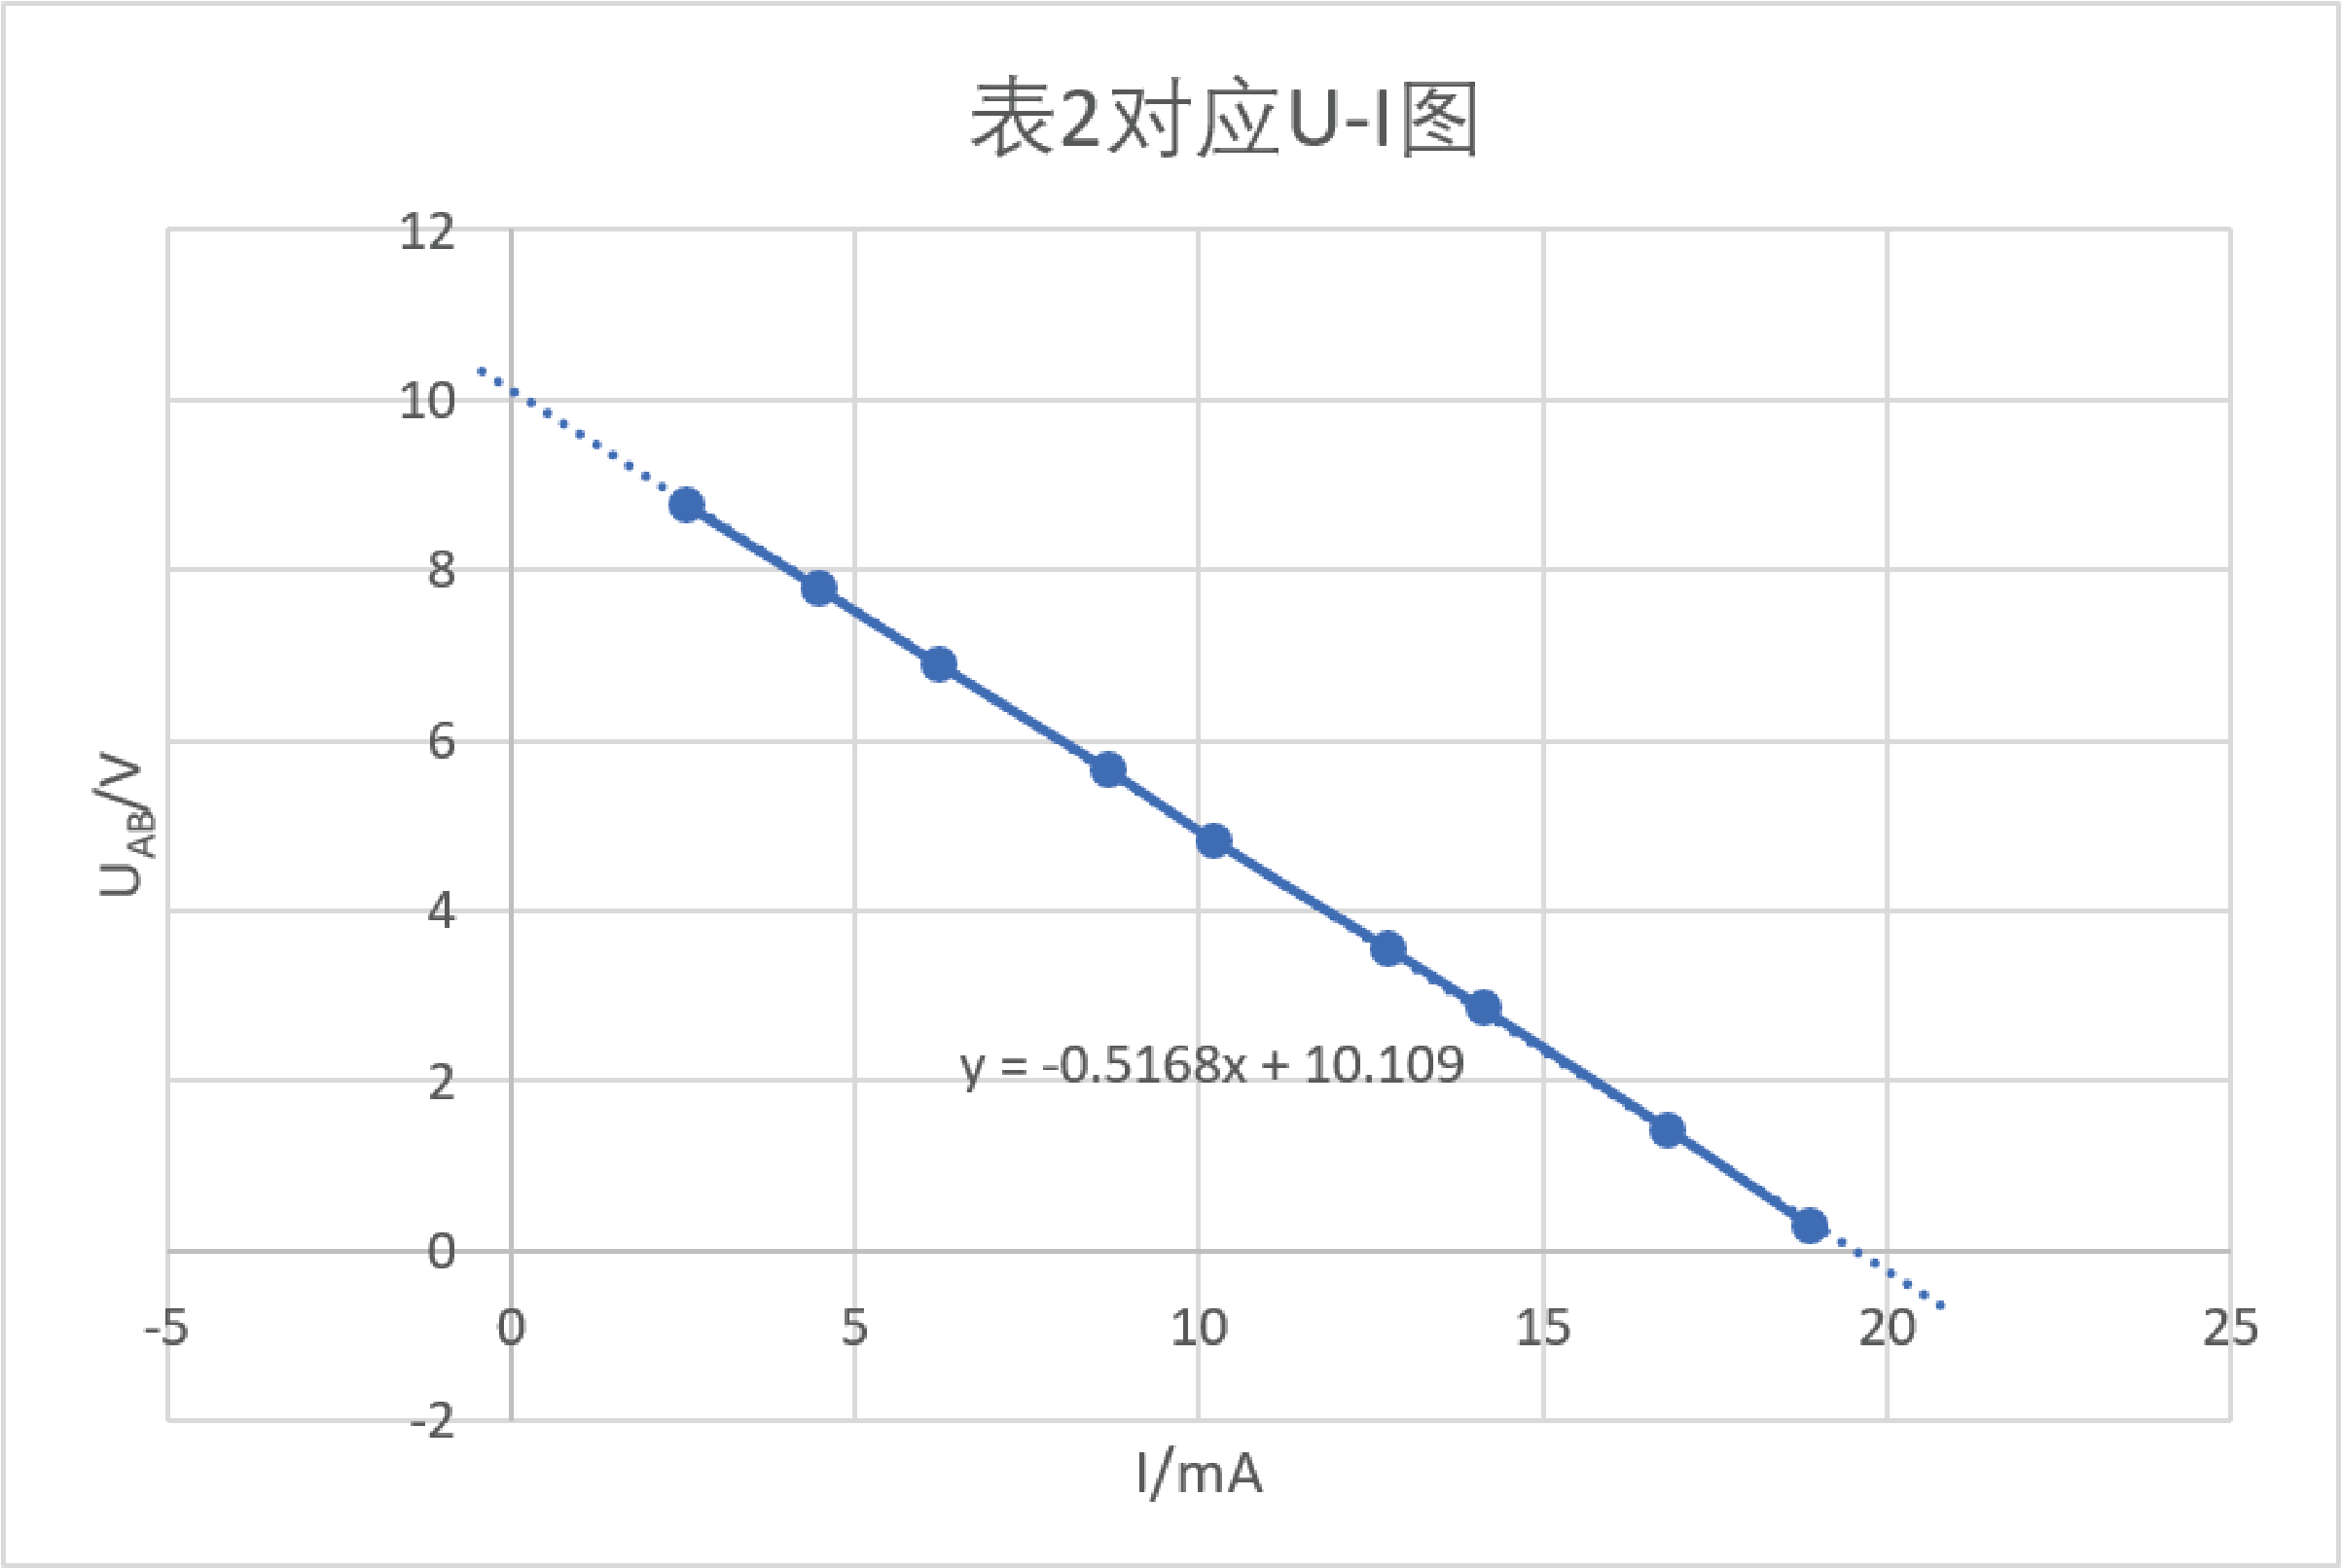
\includegraphics[scale=0.35]{图1}
                \caption{原电路\label{fig:1}}
            \end{minipage}
            \qquad
            \begin{minipage}[t]{0.5\textwidth}
                \centering
                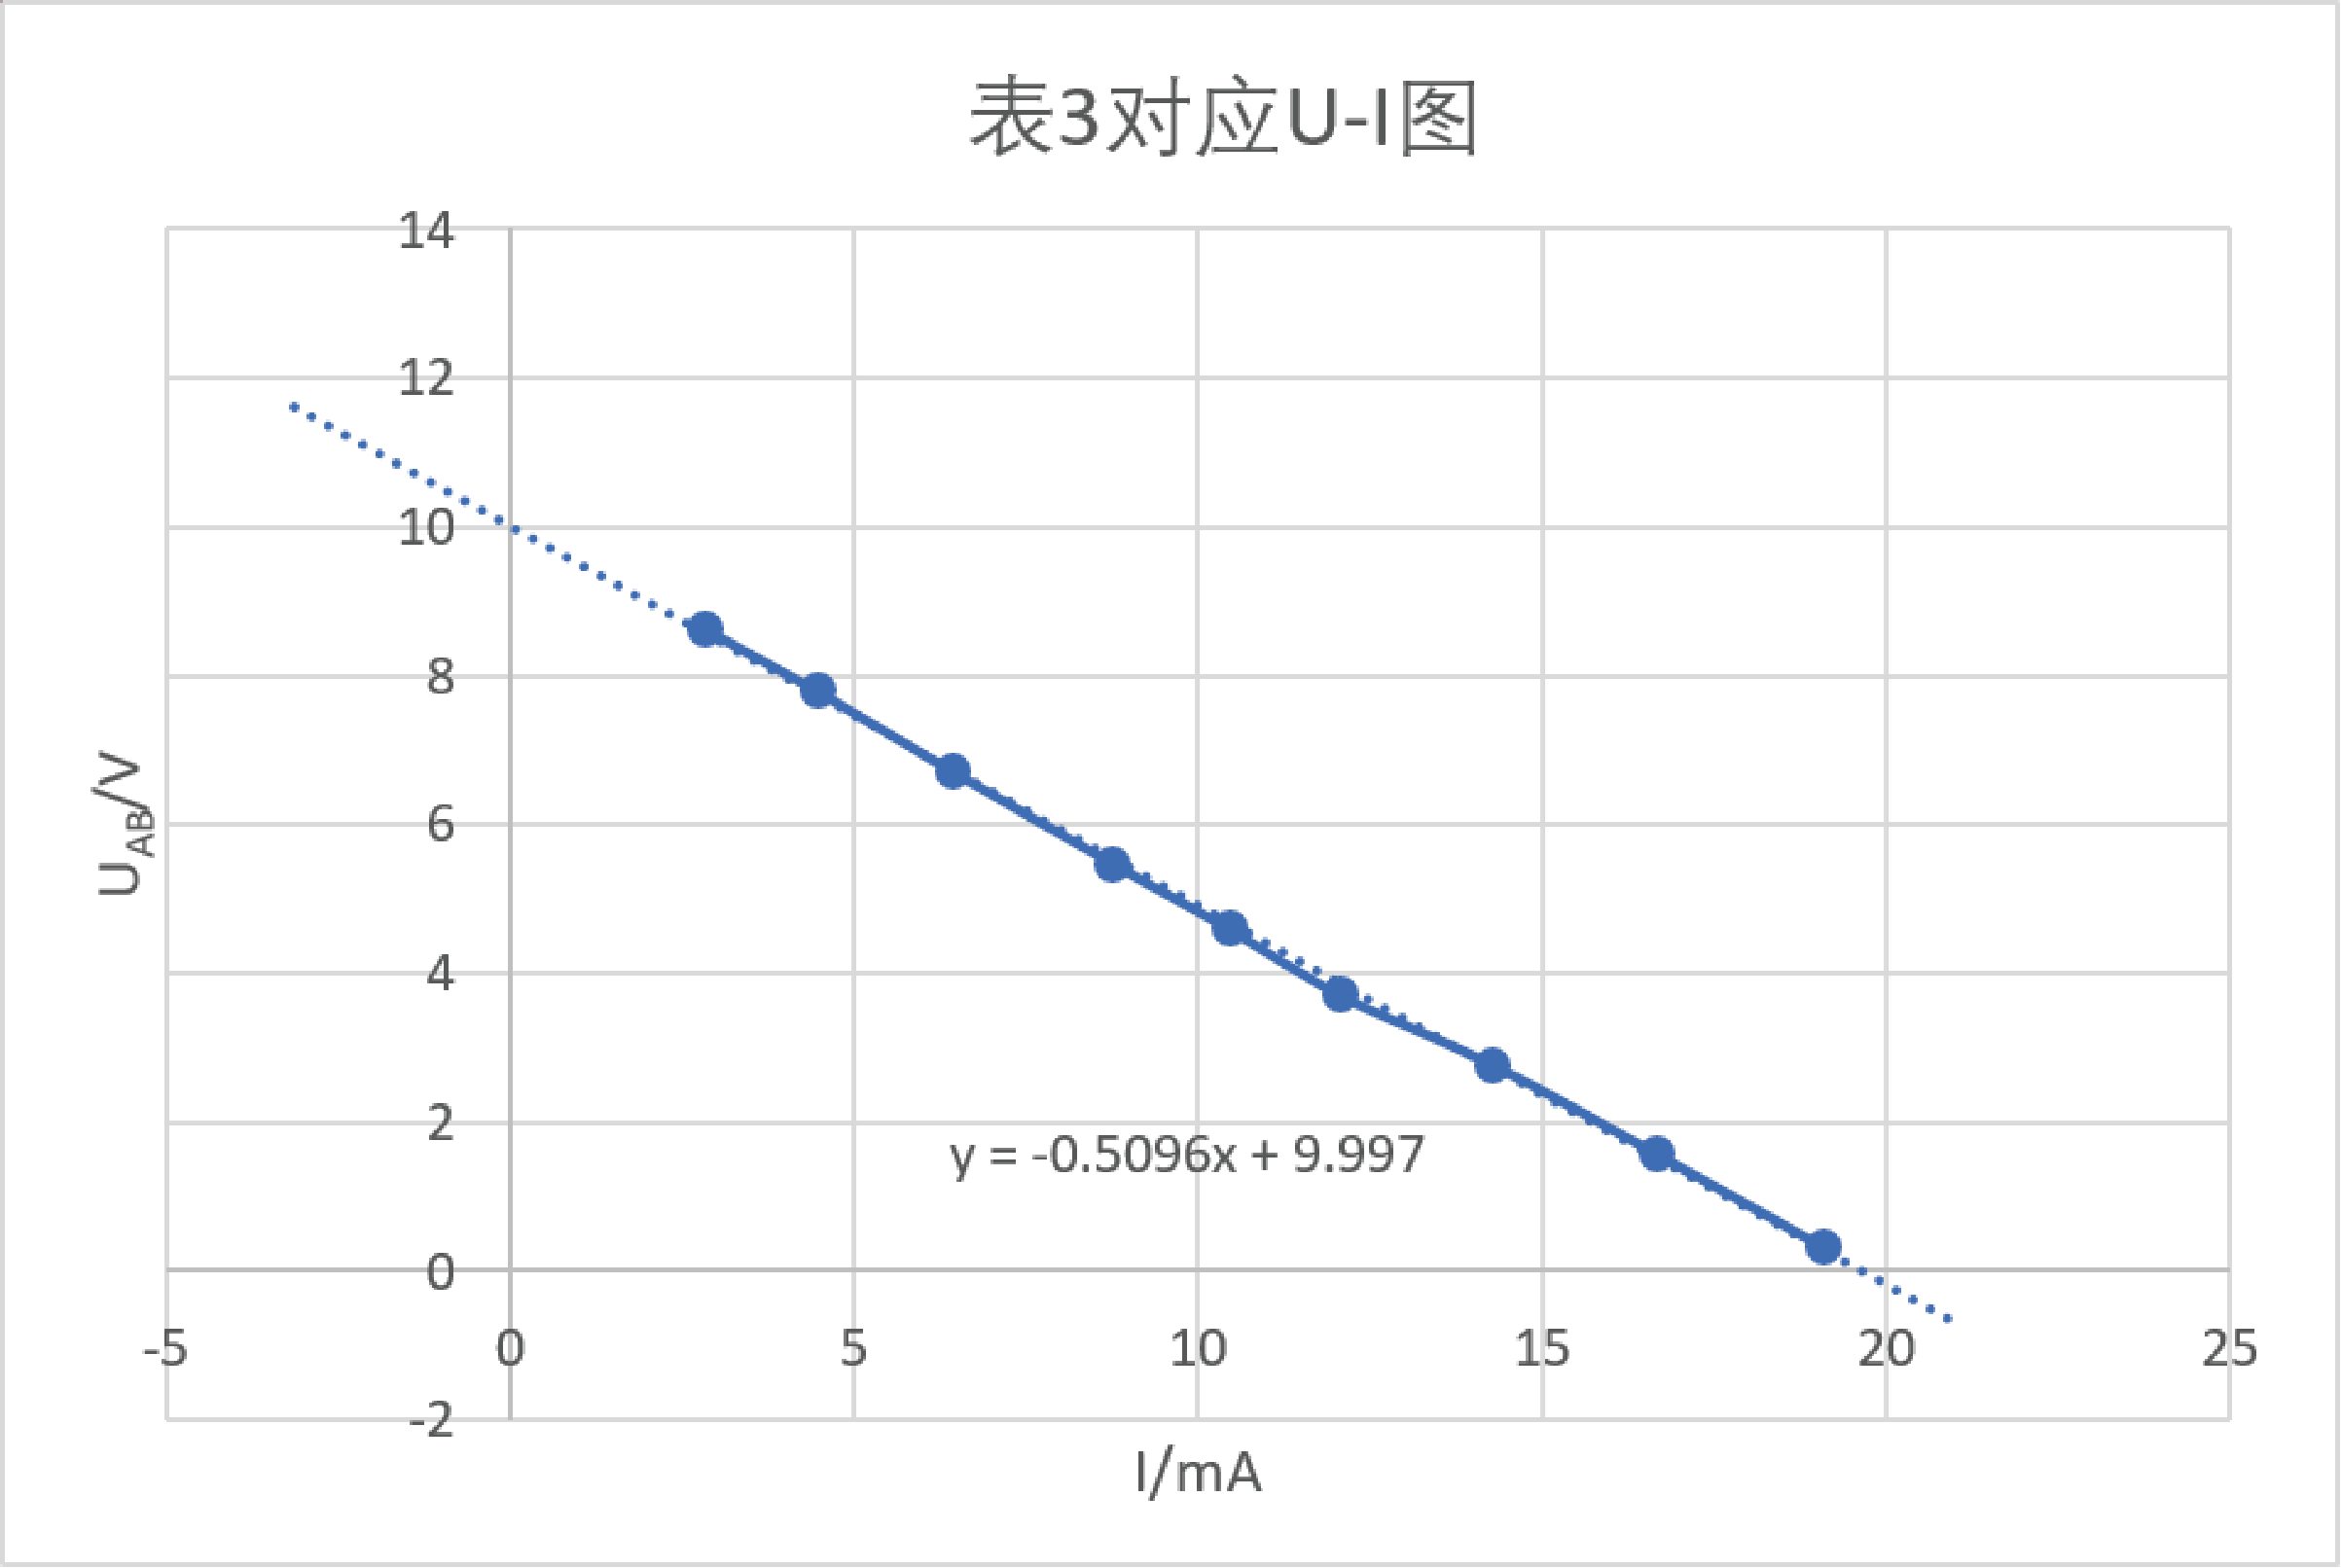
\includegraphics[scale=0.35]{图2}
                \caption{戴维南等效电路\label{fig:2}}
            \end{minipage}
        \end{figure}
        \subsection{实验结果}
        戴维南定理成立。
    \section{讨论、心得}
            通过本次实验,我更加直观的认识了戴维南定理的正确性,明白了戴维南定理在电路分析方法的重要性。
    \section{思考题}
            \begin{enumerate}
                \item 在求戴维南或诺顿等效电路时,做短路实验,则测$I_{SC}$的条件是什么?在本实验中可否直接做负载短路实验?实验前对线路图 1 预先做好计算,以便调整实验线路及测量时可准确地选取电表的量程。
                \par 条件:有源二端口网络的内阻不能太小,否则会产生很大的电流。本实验有源二端网络的内阻较大,可以直接做负载短路实验。
                \item 简述测量有源二端口网络开路电压及等效内阻的几种方法,并比较其优缺点。 
                \par  
                \begin{enumerate}
                    \item 开路电压、短路电流法测$R_o$。在有源二端口网络输出端开路时,用电压表直接测出其输出端的开路电压$U_{OC}$,然后再将其输出端短路,用电流表测其短路电流$I_{SC}$,其等效内阻为$R_o = \frac{U_{OC}}{I_{SC}}$。如果二端口网络的内阻很小,若将其输出端短路则易损坏其内部元件,因此不宜用此法。
                    \item 伏安法。用电压表、电流表测出有源二端口网络的外特性曲线如下图。根据外特性曲线输出斜率,则内阻为$R_o = \frac{U_{OC} - U_N}{I_N}$其中,额定值$I_N$时的输出端电压值为$U_N$。此法与法a相比,不容易破坏电路元器件,但是操作更加复杂。
                    \begin{center}
                        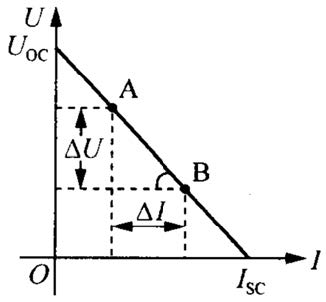
\includegraphics[scale=0.8]{伏安特性}
                    \end{center}
                    \item 半电压法测$R_o$。如图所示,当负载$R_L$的电压为被测网络开路电压的一半时,负载电阻即为被测有源二端口网络的等效内阻值。此法相对法b较简单,但是需要额外电阻箱或电位器,成本较高。
                    \begin{center}
                        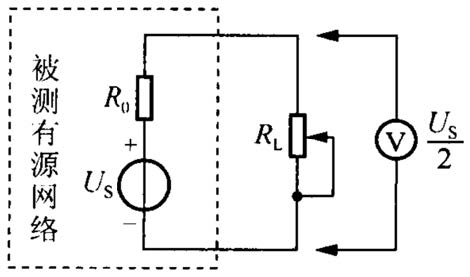
\includegraphics[scale=0.8]{半电压}
                    \end{center}
                \end{enumerate}
            \end{enumerate}
\end{document}